\chapter{Análise Bibliográfica sobre Redes Neurais e Deep Learning Aplicadas em Jogos, por Arthur Couto\label{chap:bibliometria:CrimsonCrown}}

\section{Planejamento do estudo}
Esse trabalho tem o intuito de treinar o uso da técnica de análise bibliométrica para fins didáticos, e no caso dessa pesquisa específica, servir para o autor como uma introdução ao mundo de pesquisas científicas sobre redes neurais e suas potenciais aplicações.

A pesquisa foi feita com o intuito de responder as seguintes questões:

\begin{itemize}
    \item O que é produzido cientificamente com relação a redes neurais, especificamente aplicadas a jogos?
    \item Quais são os tópicos mais frequentemente relacionados a essas pesquisas?
    \item Quais são os focos do desenvolvimento científico dessa área?
\end{itemize}

As duas primeiras perguntas são referentes a estrutura conceitual de redes neurais, enquanto a terceira pergunta é referente à estrutura social desse tópico.

Essas perguntas podem ser respondidas por meio de uma pesquisa bibliométrica. O método utilizado será o descrito em \citet{aria_bibliometrix_2017}, como especificado na sessão 5.8 deste documento, utilizando o pacote Bibliometrix e a interface Biblioshiny como ferramentas para a análise.

\section{Coleta de dados}
Os dados foram coletados na Web of Science no dia 8 de fevereiro de 2022, acessado por meio do Portal de Periódicos da CAPES.

A query de busca utilizada foi ((\textit{deep learning})OR(\textit{neural network}))AND \textit{game} (\textit{all fields}). Os termos \textit{deep learning} e \textit{neural network} tentam pegar artigos que usam esses métodos, e o termo \textit{game} tenta pegar uma aplicação específica. A conjunção AND faz com que os artigos obtidos sejam relacionados tanto com métodos de redes neurais ou \textit{deep learning} quanto com jogos.

Essa \textit{query} obteve 4547 resultados, porém apenas os primeiros 1000 foram exportados. A exportação foi feita utilizando a opção de exportar em formato BibTeX, \textit{records from 1 to 1000}, \textit{custom selection} com todos os campos selecionados. Uma tentativa de exportar 4547 resultados causou um arquivo com apenas 50 registros, por isso a opção de exportar apenas os primeiros 1000 foi utilizada.

\section{Análise dos dados}
Os 1000 documentos obtidos durante a coleta de dados incluíam vários tipos de documentos, mas apenas os artigos científicos publicados nos interessam. Após filtrar todos os outros tipos de documentos, sobraram apenas 412 artigos. Esse será o \textit{dataset} utilizado, e o chamaremos de NeuralNetworkGame/Artigos, ou NNGA@CrimsonCrown.

A figura \ref{fig:CrimsonCrown:NNGA:CoOcurrence} mostra a rede de coocorrências das palavras-chave encontradas nos artigos do \textit{dataset} NNGA@CrimsonCrown.

\begin{figure}
    \centering
    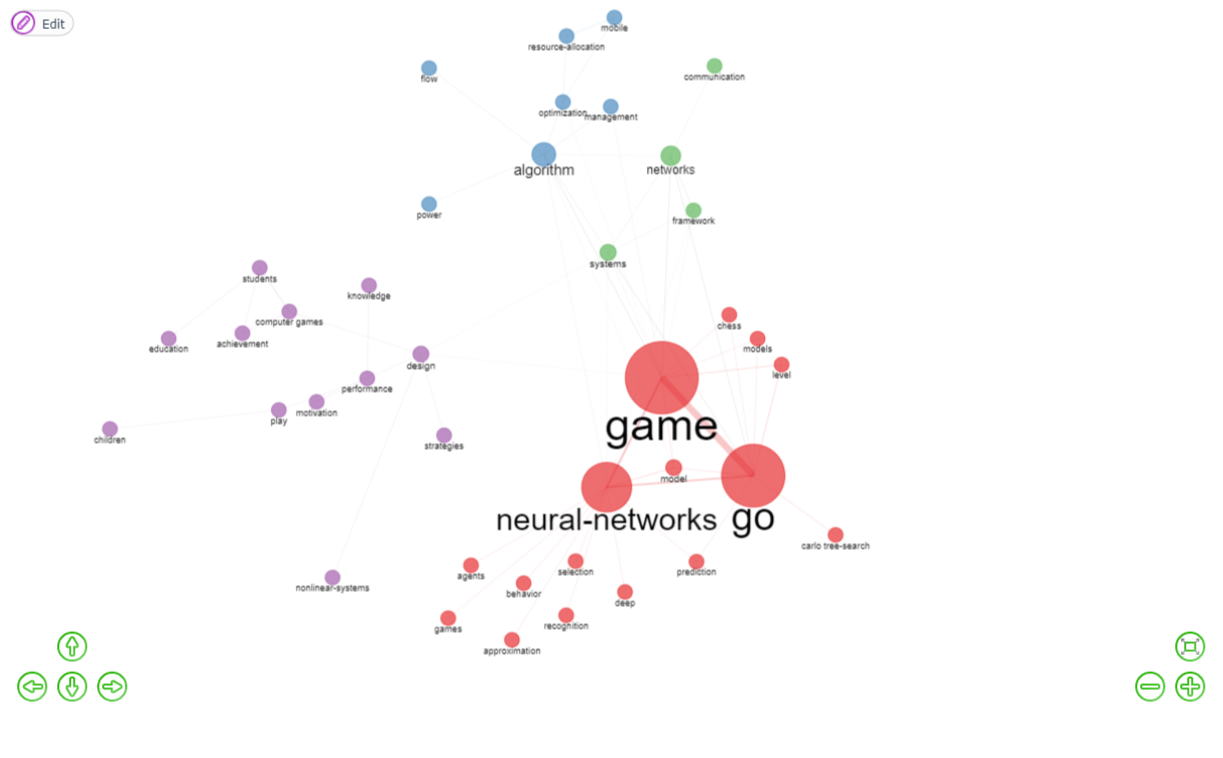
\includegraphics[angle=0,width=1\textwidth,height=0.5\textheight]{experiments/CrimsonCrown/AnaliseBibliometrica/RedesNeuraisJogos/NNGAConceptNetwork.png}
    \caption{Rede de coocorrências das palavras-chave dos artigos do \textit{dataset} gerado no biblioshiny, com alterações para facilitar visualização.}
    \label{fig:CrimsonCrown:NNGA:CoOcurrence}
\end{figure}

Pode ser observado que os dois maiores pontos são \textit{neural-networks}, go e \textit{game}. Faz sentido que os termos de busca sejam prevalentes, mas a presença de go como palavra chave tão comum é interessante. Isso pode ser explicado pelo fato de que go é um jogo que foi muito estudado em conjunto com redes neurais, e é um caso de teste simples e poderoso, já que sua árvore de possibilidades é grande demais para um algoritmo baseado em busca exaustiva conseguir bons resultados em uma quantidade razoável de tempo. Na figura \ref{fig:CrimsonCrown:NNGA:ThematicMap} go foi classificado como um tema de base para essa área do conhecimento, o que fortalece a ideia de que go é comummente utilizado como caso de teste base para estudos em redes neurais.

\begin{figure}
    \centering
    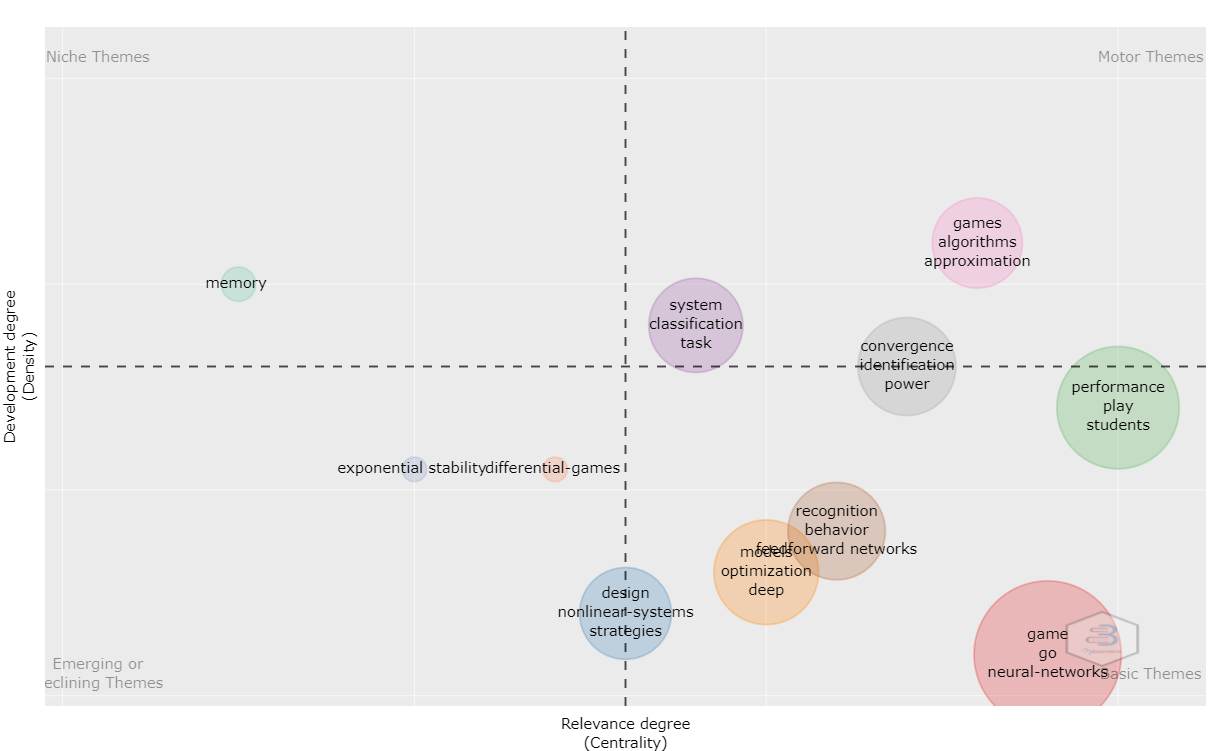
\includegraphics[angle=0,width=1\textwidth,height=0.5\textheight]{experiments/CrimsonCrown/AnaliseBibliometrica/RedesNeuraisJogos/NNGAThematicMap.png}
    \caption{Mapa temático das palavras-chave dos artigos do \textit{dataset} gerado no biblioshiny.}
    \label{fig:CrimsonCrown:NNGA:ThematicMap}
\end{figure}

Para tentar responder à terceira pergunta do estudo, o \textit{three-field plot} da figura \ref{fig:CrimsonCrown:NNGA:TFP} foi gerado. Nele podemos observar a predominância de autores da China, com Estados Unidos da América e Reino Unido sendo dois grandes focos também.  

\begin{figure}
    \centering
    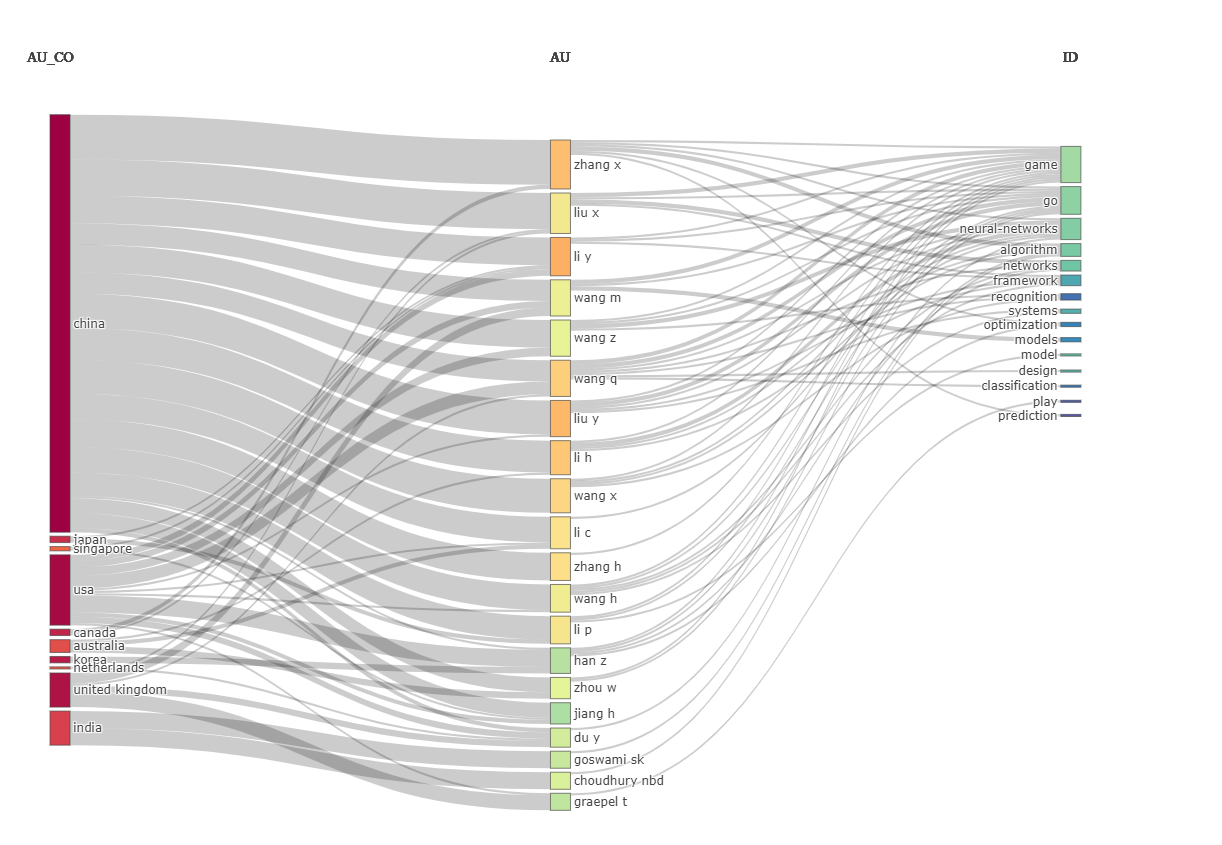
\includegraphics[angle=0,width=1\textwidth,height=0.5\textheight]{experiments/CrimsonCrown/AnaliseBibliometrica/RedesNeuraisJogos/NNGASankeyAuCoKW.png}
    \caption{\textit{Three-Field Plot} do \textit{dataset} NNGA@CrimsonCrown, com 20 autores, países e palavras-chave mais proeminentes.}
    \label{fig:CrimsonCrown:NNGA:TFP}
\end{figure}